% !TEX root = thesis.tex

\chapter{TraffickCam}
\label{ch:3}
Sex trafficking has become more prevalent as the Internet provides new avenues for the recruiting, advertisement and sales of sexual services~\cite{kunze2009sex}. We explore the opportunities of a highly connected world to build tools to fight sex trafficking. We particularly focus on understanding places where large scale image collection and analysis offers new investigative tools.

Images are a common way to advertise sex services. Images are interesting from an investigative standpoint because they connect the person in the image to the location where the image was taken. Therefore, they can help to characterize where a particular person was at different times. In the context of a sex trafficking investigation, this can be used to
directly confirm that a person was in different states or countries. Among other things, this can change the set of laws under which a trafficker can be prosecuted.

We aim to create a database of hotel room images that an investigator can use to understand the pictures they may acquire during a sex trafficking investigation. We build a dataset from publicly shared imagery on hotel booking sites, as well as from a smartphone app to crowd-sourcing the collection of pictures of hotel rooms. The crowd-sourcing option
takes advantage of large scale trends in how people use social media; approximately 350 million photos are uploaded daily to Facebook. Tapping into this already common behavior creates the potential to rapidly create a relatively comprehensive, distributed,
and continually updated resource that details the current appearance of hotel rooms worldwide.

\section{Dataset Creation}
In order to have the highest likelihood of finding a good feature match between a investigator's query image and the images in our dataset, our dataset should have as many images of as many rooms in as many hotels as possible. Additionally, it should have images from as many different times as possible. Hotels regularly renovate and change their internal appearance, meaning that photographs in our dataset may become outdated. These outdated images may still be valuable, however, in pinpointing the time frame in which an individual was trafficked (e.g., ``This photograph was taken before the 2015 renovations, which means the person in the photograph was a minor at the time the advertisement was placed.'').

\section{Crowd-sourced Image Collection}
\begin{figure*}[ht!]
  \begin{center}
    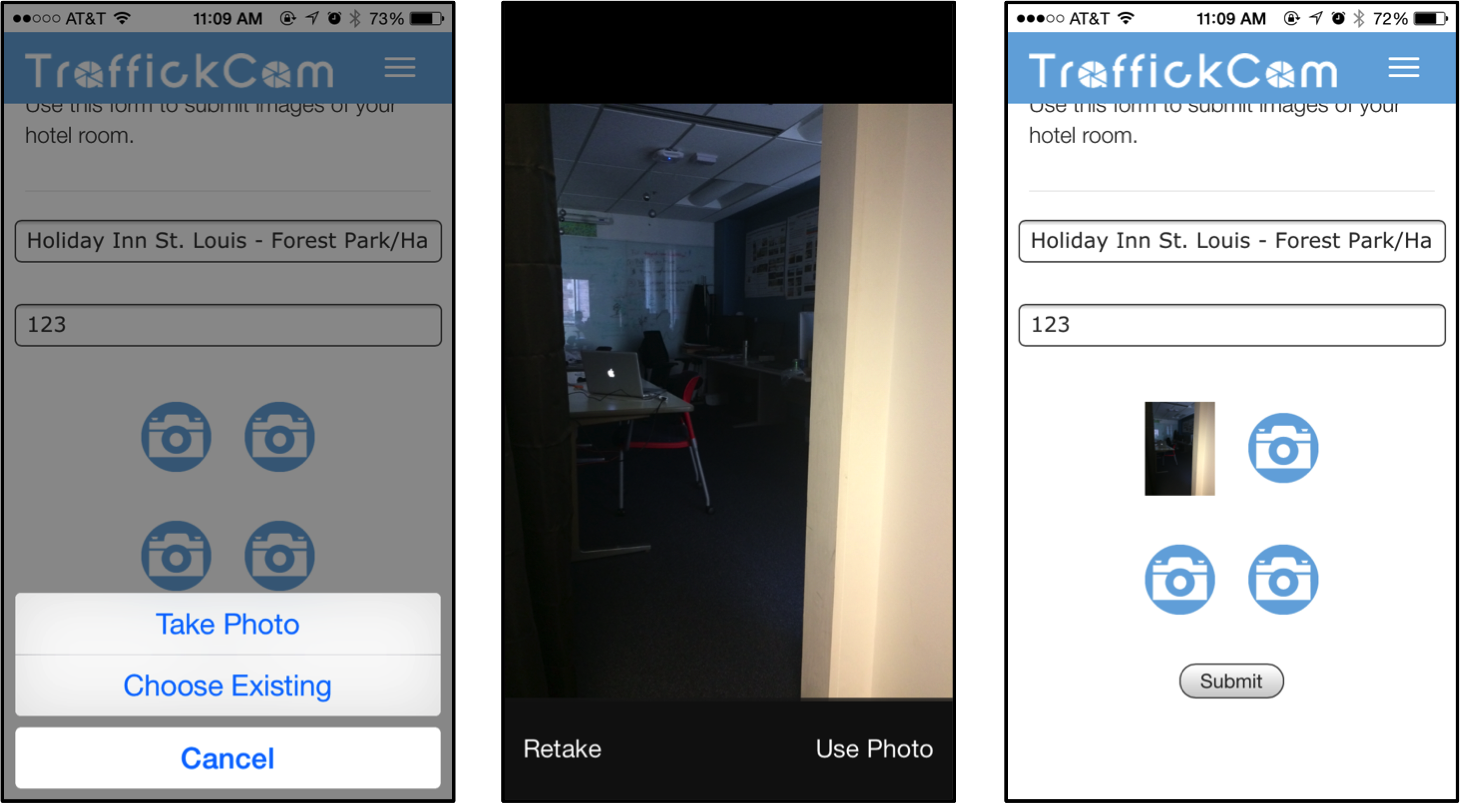
\includegraphics[width=\textwidth]{figures/chapter3/appScreenshots.png}
  \end{center}
  \caption[Smartphone app screenshots.]{Screenshots of the smartphone app, TraffickCam, that allows anyone to contribute to the database. The app is designed to require minimal user time and to protect the user's identity.}
  \label{fig:appScreenshots}
\end{figure*}

We take two approaches to populating our dataset of hotel room images. First, we utilize already existing datasets of hotel room images used for marketing and travel sales. In particular, we keep track of the millions of images made available through Expedia’s Affiliate Network API (http://developer.ean.com/) and create a reference in our database to the original data and its associated metadata. These photos, however, are often provided by the hotels themselves and may not present a comprehensive view of the hotel itself (e.g., only the nicest rooms from good angles in the best lighting). They may also not be updated following renovations. Both of those flaws would be problematic if these photographs were the only representations our dataset had of these hotels. 

To supplement the images captured from existing datasets, we have created a smartphone based crowd-sourcing application named TraffickCam, which allows travellers to upload their own photographs of a hotel room. This application is shown in Figure~\ref{fig:appScreenshots}. Users are asked to provide minimal information regarding the photo -- the name of the hotel they're staying in and their room number, along with images of the room.

The application, called TraffickCam, is available from the iOS and Android stores, in addition to being accessible via any modern browser at \url{http://traffickcam.org}.

Figure~\ref{fig:example_ims} demonstrates the importance of collecting images from the TraffickCam application. Images from publicly available sources such as Expedia are professionally photographed and showcase the nicest, staged rooms at a hotel. Images posted in ads for sex services are often taken with a smart phone by the victim themselves in less impressive hotel rooms. The TraffickCam images are often more representative of the types of photos seen in these ads. In addition, the TraffickCam photos provide an ever-growing archive of what the hotel looked like at a giving time, capturing renovations and changes that may not be present in the images on travel websites.

\begin{figure*}[ht!]
  \begin{center}
  \begin{subfigure}[b]{\textwidth}
    \centering
    ~~~~~~~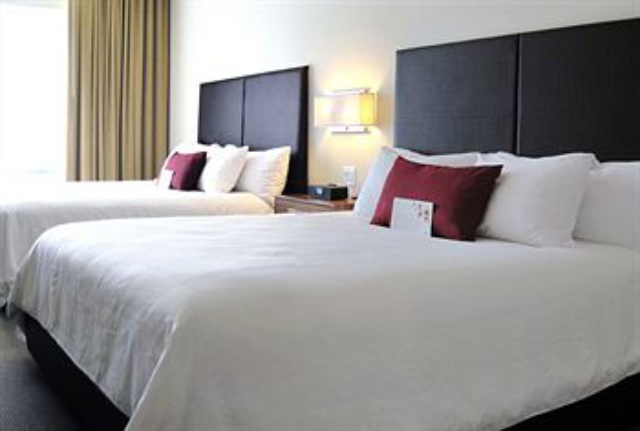
\includegraphics[width=.25\columnwidth]{figures/chapter3/expediaIms/1.jpg}
    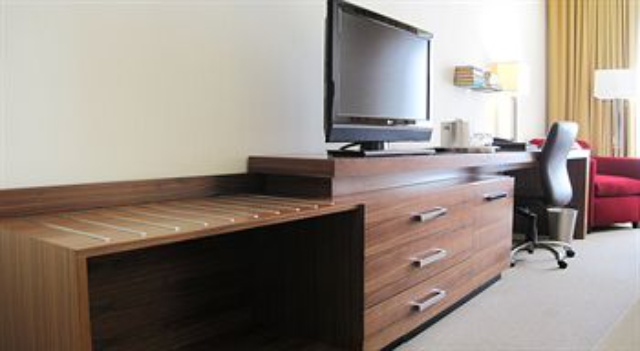
\includegraphics[width=.25\columnwidth]{figures/chapter3/expediaIms/2.jpg}
    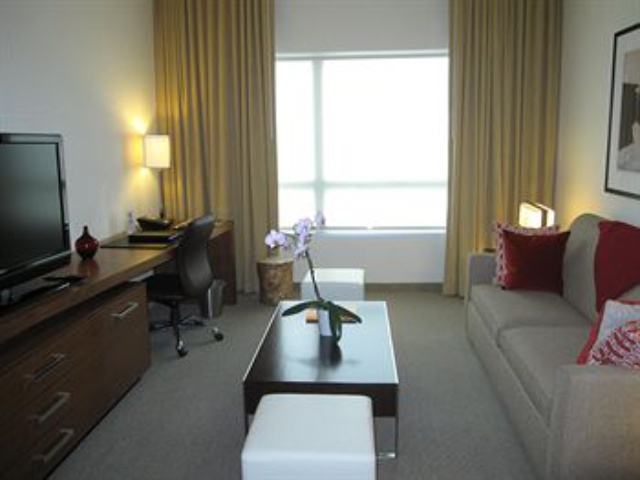
\includegraphics[width=.25\columnwidth]{figures/chapter3/expediaIms/3.jpg}
    \newline
    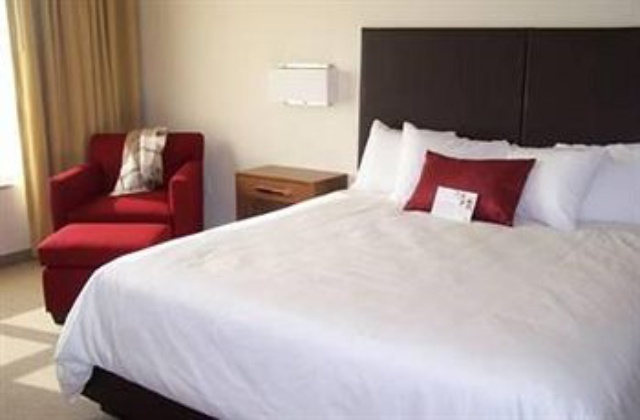
\includegraphics[width=.25\columnwidth]{figures/chapter3/expediaIms/4.jpg}
    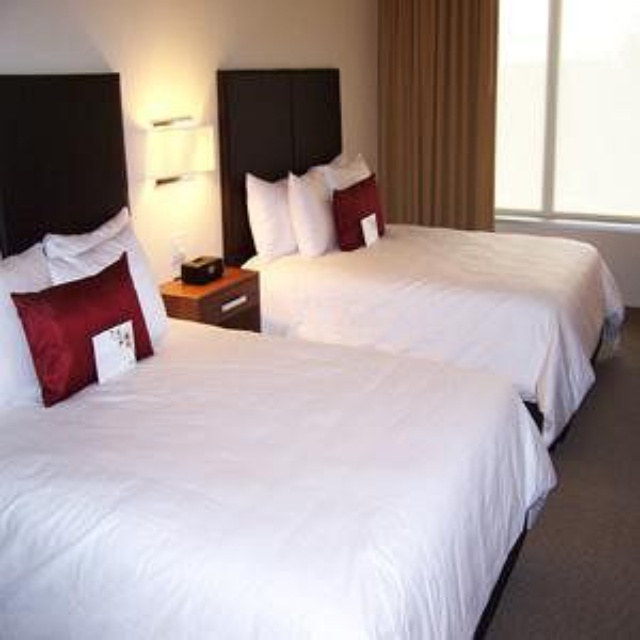
\includegraphics[width=.25\columnwidth]{figures/chapter3/expediaIms/5.jpg}  
    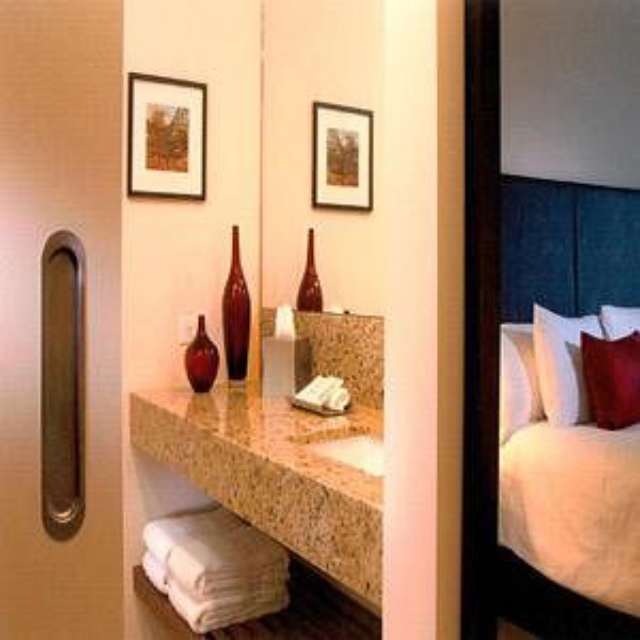
\includegraphics[width=.25\columnwidth]{figures/chapter3/expediaIms/6.jpg} 
    \caption{Expedia Images}
  \end{subfigure}
  
  \begin{subfigure}[b]{\textwidth}
    \centering
    ~~~~~~~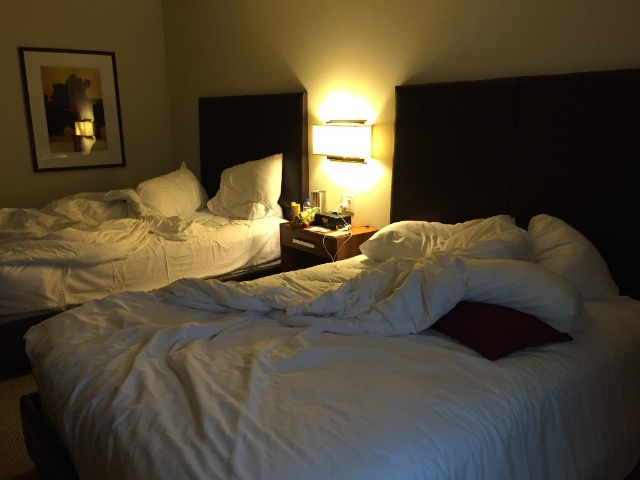
\includegraphics[width=.25\columnwidth]{figures/chapter3/traffickCamIms/1.jpg}
    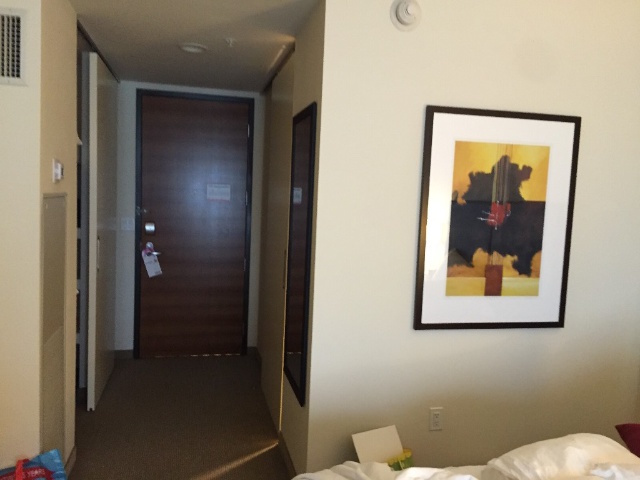
\includegraphics[width=.25\columnwidth]{figures/chapter3/traffickCamIms/2.jpg}
    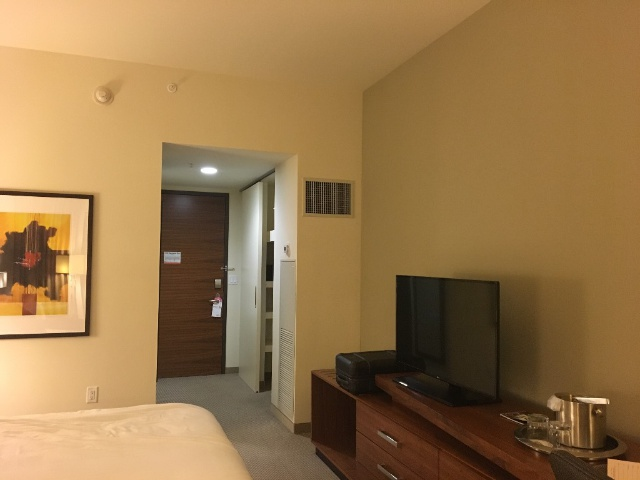
\includegraphics[width=.25\columnwidth]{figures/chapter3/traffickCamIms/3.jpg}
    \newline
    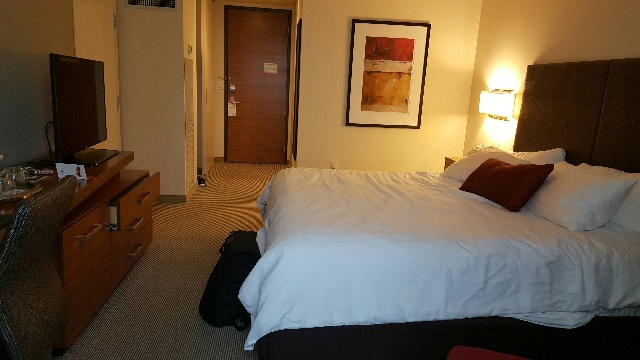
\includegraphics[width=.25\columnwidth]{figures/chapter3/traffickCamIms/4.jpg}
    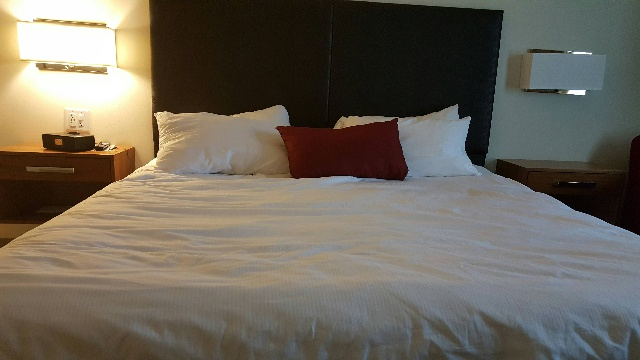
\includegraphics[width=.25\columnwidth]{figures/chapter3/traffickCamIms/5.jpg}  
    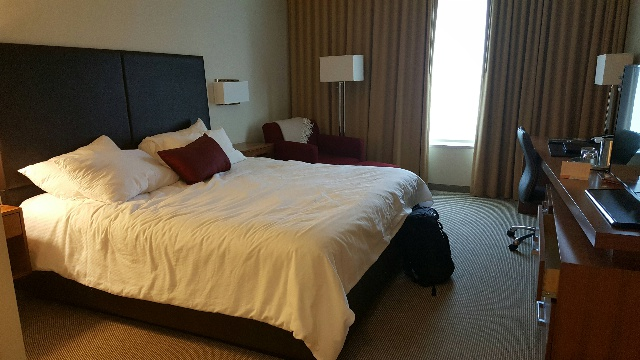
\includegraphics[width=.25\columnwidth]{figures/chapter3/traffickCamIms/6.jpg}  
    \caption{TraffickCam Images}
  \end{subfigure}
  
  \begin{subfigure}[b]{\textwidth}
  \centering
    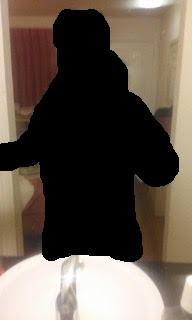
\includegraphics[height=120px]{figures/chapter3/backpage/3.jpg}
    ~~~~~~
    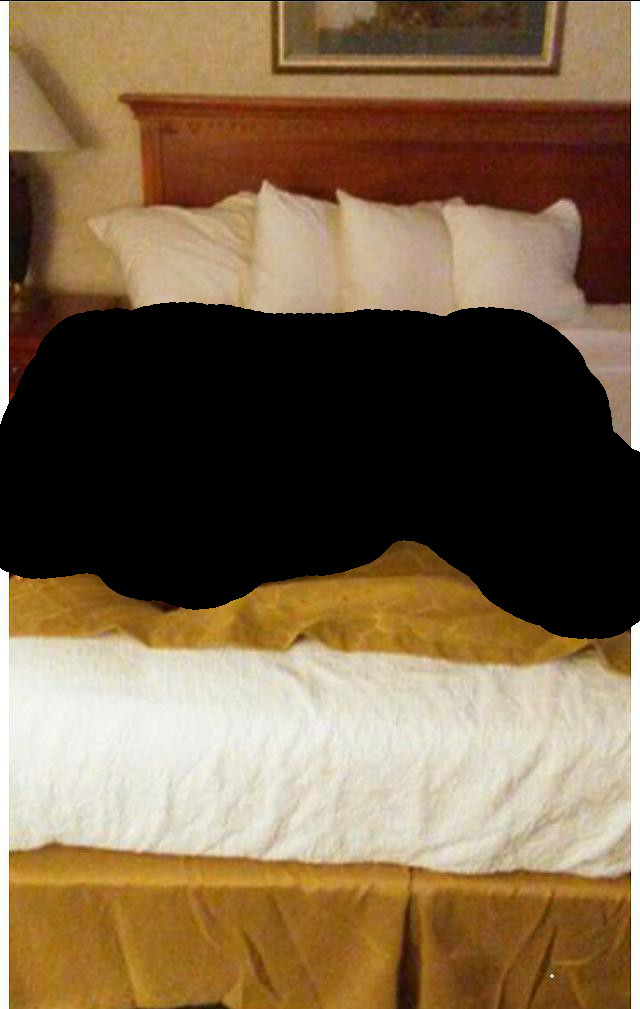
\includegraphics[height=120px]{figures/chapter3/backpage/1.jpg}
    ~~~~~~
    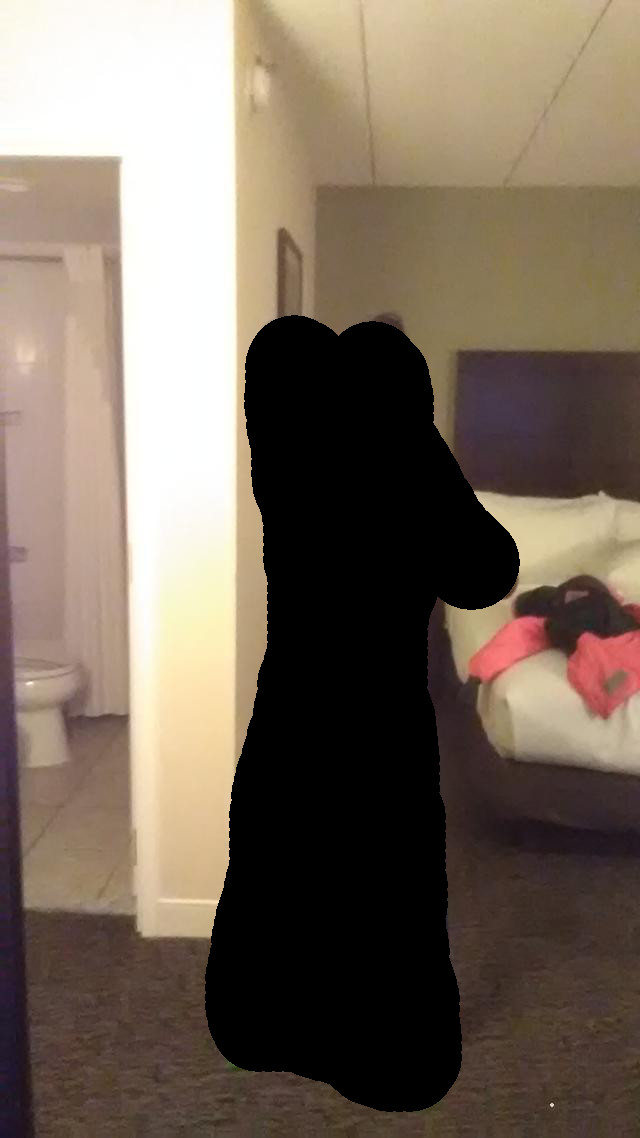
\includegraphics[height=120px]{figures/chapter3/backpage/2.jpg}
    \caption{Example Censored Query Images from Law Enforcement}
  \end{subfigure}
  
  \caption[Example images from TraffickCam and Expedia.]{The top set of images are from Expedia and the middle set of images taken by TraffickCam users at the same hotel. The bottom set of images are censored versions of the types of images that might be provided by law enforcement. These examples demonstrate the discrepancy in the types of photos provided by Expedia, by the TraffickCam app and by law enforcement.}
  \label{fig:example_ims}
  \end{center}
\end{figure*}

\section{Dataset Scope}
Today, the TraffickCam smart phone app has been downloaded by over 100,000 users on both iOS and Android devices. The application, shown in Figure~\ref{fig:appScreenshots}, simply requires users enter their hotel name, room number and take up to four images of their hotel room and bathroom. Users remain anonymous, submitting only their GPS location so that the system can verify that the photos were taken at the same location as the hotel (a protection against both malicious uploads of erroneous photos and accidental uploads due to the user selecting the incorrect hotel). Many crowdsourcing platforms help encourage the ongoing engagement of their community using points or sticker systems, or otherwise providing the user with information about how much they've contributed to the community. Because our users are entirely anonymous, however, we have no details about a user's submission history. Instead, we encourage ongoing engagement by providing the user with insight on how their most recent submission contributed to the dataset as a whole (e.g., the total number of photos including their most recent submission, the number of photos submitted so far on that day, or the number of photos previously submitted at that hotel). These types of feedback messages are seen in Figure~\ref{fig:appScreenshots}.

Since TraffickCam was publicly released for iOS and Android in June 2016, TraffickCam users have uploaded over 188,000 images from nearly 27,000 hotels around the world. In addition to this ongoing collection of photos, the dataset also includes images from publicly available sources of hotel room photos, such as those available via the Expedia Affiliate Network~(\url{http://developer.ean.com/}). As of October 2017, there are over 2.85 million images from over 254,000 hotels represented in the TraffickCam dataset.

While the TraffickCam application purposefully collects no identifiable information about users to protect them from any legal action, we are able to estimate the number of users per hotel by the timestamp of the images uploaded -- the application asks users for a set of four images, so we assume images that are disjoint in time are from different users.

\section{Implementation Details}
We have implemented a RESTful API in Python Django, a web framework for rapid web development. Django handles the interaction between the server side code, web front end code, MySQL database and Apache web server. Test, stage and production Ubuntu environments are hosted through Amazon Web Services.

The iOS app, available through the Apple App Store, is simply a container that renders an HTML5+jQuery+AJAX web application hosted on~\url{https://traffickcam.org}, rather than a full native application. This allows for rapid development and easy exploration of different user experience choices (e.g., different motivational messages to display to users upon submission). The Android application is a native application available on the Google Play store.

\section{Application Statistics}
Since TraffickCam was released in December of 2015, there have been 68,700 installations on iOS devices and 28,500 installations on Android devices. These installations are primarily from users in the United States, where the search tool will first be deployed for law enforcement, but also include several thousand installations each from Europe and Asia. On average since the advertised release of the TraffickCam applications for iOS and Android in June of 2016, users have submitted just over 530 images a day.

\begin{table*}[t!]
  \begin{center}
    \begin{tabular}{*{15}{c}}
    \hline
    Feature Set & Top 1 & Top 10 & Top 20 \\
    \hline
    SIFT & \textbf{0.44} & \textbf{0.66} & \textbf{0.69} \\
    Places (fc6) & 0.32 & 0.63 & \textbf{0.69} \\
    Places (fc7) & 0.26 & 0.54 & 0.65 \\
    Places (fc8) & 0.14 & 0.44 & 0.52 \\
    Places (output) & 0.04 & 0.25 & 0.31
    \end{tabular}
  \end{center}
  \caption{Results with baseline feature matching methods. SIFT feature matching performance is better than features extracted from Places in identifying the correct hotel in the single most similar image (Top 1). SIFT features and features extracted from Places~(`fc6') have similar performance in identifying the correct hotel in the Top 10 and Top 20 most similar images.}
  \label{tab:results}
\end{table*}

\section{Preliminary Results}
\label{methodology}
We explore two baseline approaches for matching a query image to TraffickCam images. The first approach is based on SIFT feature matching~\cite{lowe1999object}, and the second approach is based on matching features extracted from the last fully connected layer of the pre-trained Places network~\cite{zhou2014places}.

In the first approach, we extract SIFT features from every image in the dataset. Given a query image, we extract SIFT features. For each of those features, we find the $n$ nearest neighbors in the set of features extracted from the database of images using the VLFeat MATLAB implementation of FLANN's KD-Tree Forests~\cite{vedaldi08vlfeat}. Each nearest neighbor match between a feature in the query image and a feature in a database image is a ``vote'' that the query image was taken in the same hotel as the database image. Votes are weighted by their ranking in the nearest neighbor match (e.g., the first nearest neighbor is weighted more heavily than the fifth nearest neighbor) to determine a list of candidate hotels where the query image might have been taken. This strategy is based on the approach to outdoor image localization in~\cite{Zamir10}.

In the second approach, we  extract feature representations learned from an existing deep convolutional neural network (CNN) architecture~\cite{krizhevsky2012imagenet}. We use a publicly-available, pre-trained model, which we call \emph{Places}, trained on the Places Database~\cite{zhou2014places} for scene recognition from 205 categories (e.g., airplane cabin, hotel room, shed). In this CNN architecture, features are extracted from images in a layered, feed-forward manner. Initial layers of the architecture consist of convolutions, local response normalization, local pooling, dropout layers, and rectified
linear (ReLU) activation units. The top layers of the network are four fully connected layers `fc6', `fc7', `fc8', and the final output layer `prob' that represents a categorical probability distribution. The
dimensionality of these top layers in Places are 4096, 4096, 205, and 205 respectively. In these experiments, we perform feature extraction using Caffe~\cite{jia2014caffe}, an open source deep learning framework.  

\section{Experimental Design and Results}
We explore the accuracy of the methods suggested in the previous section with a experiment based on all hotels in St. Louis.  We chose this scale of a test because in real use, investigations often have significant knowledge of where an image may be from, and because this scale makes the computational load small enough to easily test many different feature sets.

\paragraph{Test Dataset} In the St. Louis area, our database comprises 1800 images from about 200 hotels.  We break this dataset into a database and a test set as follows.  For every hotel that has at least 5 images, we choose one image as a test image and exclude it from the database.  Exactly 100 hotels fit this criteria, creating a test set of 100 images.  The 1700 remaining images were included in our database for this experiment.

\paragraph{Processing} For each query image, we follow the methodology detailed in Section~\ref{methodology}, and compute the 20 nearest neighbors in the experimental database based on each of the feature type described in the previous section.  For each query image, we find the hotel in which each of the 20 nearest neighbor images were captured, and report whether the correct hotel was in the top 1, top 5 and top 20 nearest neighbors.

\paragraph{Results} The results of this experiment are reported in Table~\ref{tab:results}. SIFT feature matching generally has the best performance, identifying an image from the same hotel as the query image as the closest match 44\% of the time. SIFT feature matching and matching using the feature extracted from Places layer `fc6' have similar performance when identifying the correct hotel in the top 10 and top 20 closest matches. The places `output' layer has generally poor performance. We show example results for SIFT feature matching in Figure~\ref{results}.

\begin{figure*}[p]
  \begin{center}
  
  \begin{subfigure}[b]{.9\textwidth}
    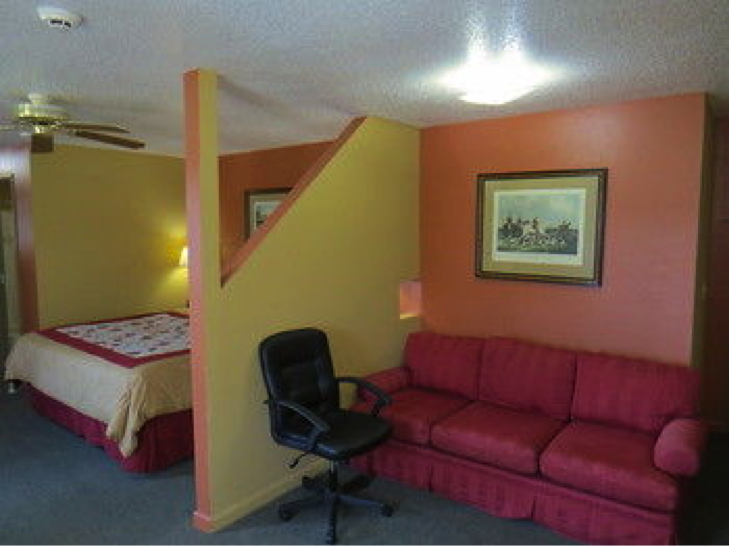
\includegraphics[width=.5\columnwidth]{figures/chapter3/good2a.png}
    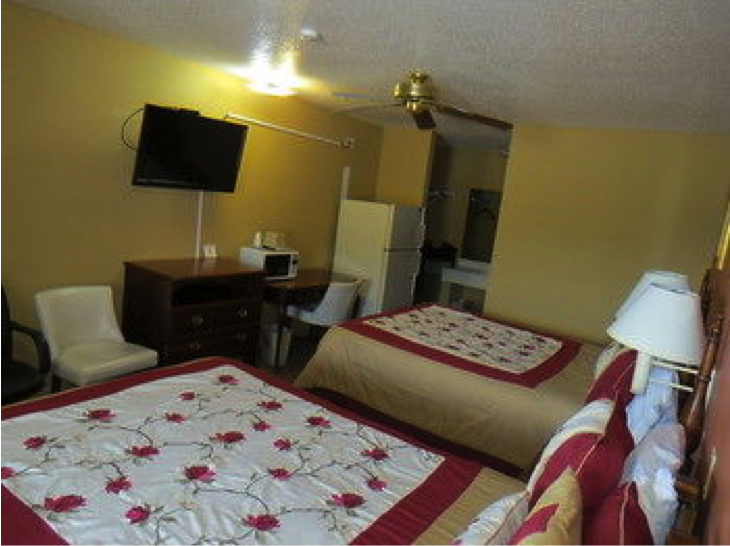
\includegraphics[width=.5\columnwidth]{figures/chapter3/good2b.png}
    \caption{A successful matching between images from dramatically different viewpoints.}
  \end{subfigure}
  
  \begin{subfigure}[b]{.9\textwidth}
    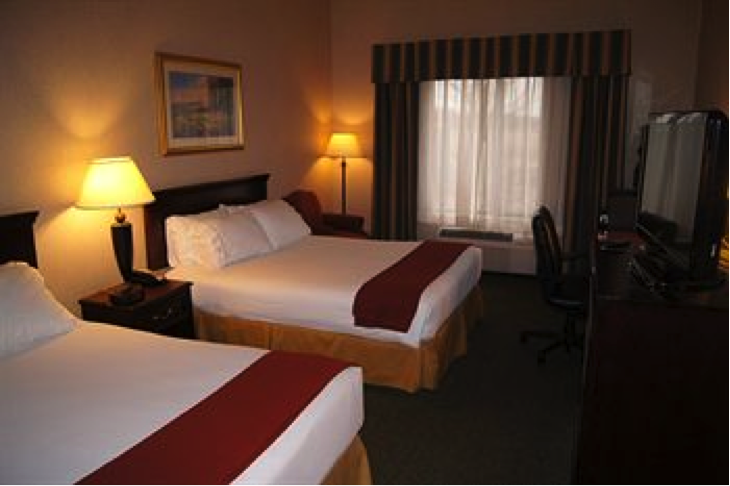
\includegraphics[width=.5\columnwidth]{figures/chapter3/good1a.png}
    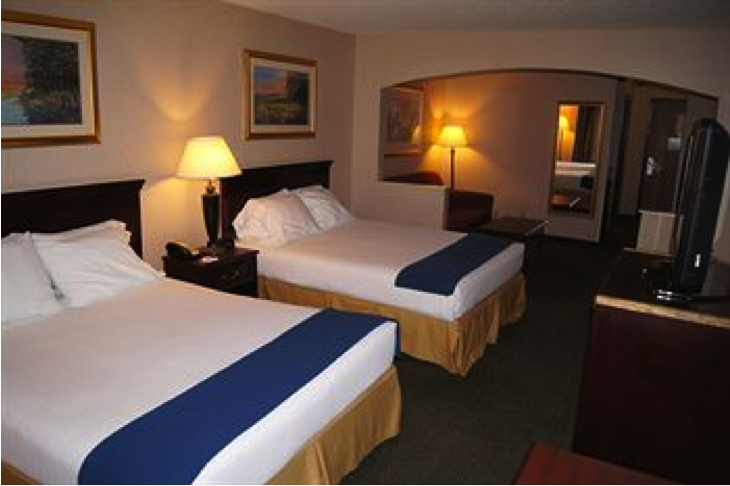
\includegraphics[width=.5\columnwidth]{figures/chapter3/good1b.png}
    \caption{A successful matching that demonstrates the limitations of our current dataset. These two images are more visually similar than we would ever expect in real world query data.}
  \end{subfigure}
  
  \begin{subfigure}[b]{.9\textwidth}
    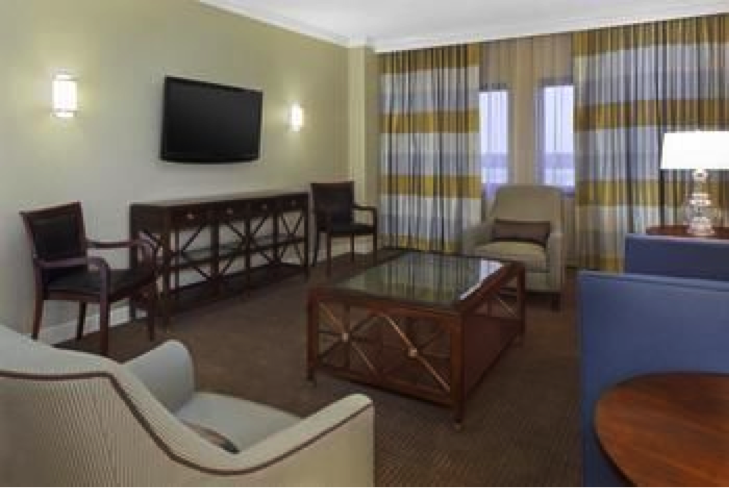
\includegraphics[width=.5\columnwidth]{figures/chapter3/bad1a.png}
    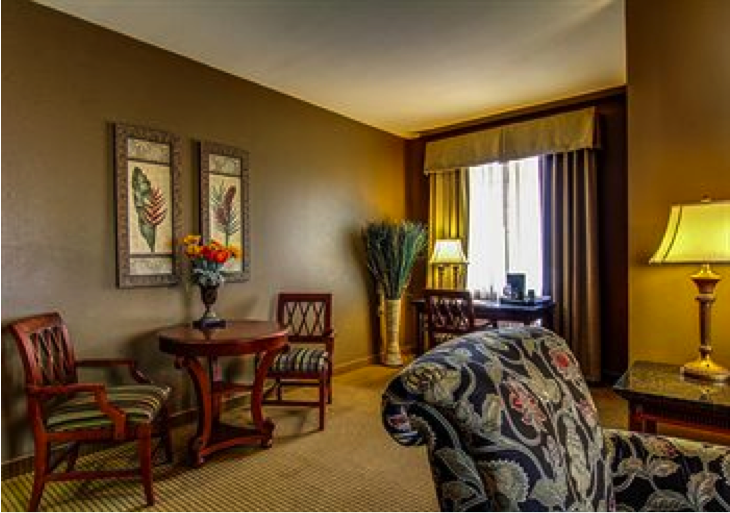
\includegraphics[width=.5\columnwidth]{figures/chapter3/bad1b.png}
    \caption{A failed matching, where SIFT feature matching found visually similar features in the furniture in hotel rooms in two different hotels.}
  \end{subfigure}
  
  \caption{The left column shows query images, and the right image shows the image which was found to be the closest match using SIFT features and the matching pipeline described in Section~\ref{methodology}. The top two rows show correctly matched pairs, where the query image and result image were taken in the same hotel. The bottom row shows an incorrectly matched pair.}
  \label{results}
  \end{center}
\end{figure*}

These preliminary results are promising on an experimental dataset that includes thousands of images from all the hotels in a city.  Qualitatively, this is a test on a scale that may itself be useful, for example if the investigation already knows to focus on a city. In Chapter~\ref{ch:5}, however, we will discuss the retrieval results of a convolutional neural network trained using the TraffickCam dataset specifically for the task of hotel recognition, and evaluated on a significantly larger, global test set with varying levels of occlusions meant to better replicate the properties of real world trafficking victim queries.